\documentclass{article}
\usepackage[a4paper, portrait, margin=1.5cm]{geometry}
\usepackage[utf8]{inputenc}
\usepackage[english]{babel}
\usepackage{longtable}
\usepackage{graphicx}
\graphicspath{ {images/} }

\title{Data Exploration of NYC Subway Dataset}
\author{Ivailo Kassamakov}
\date{October 2015}
\begin{document}

\maketitle
\begin{abstract}
The present project is an effort towards fulfilling the requirements of the Data Analyst Nanodegree at Udacity.

The goal is to perform exploratory data analysis on a dataset collected from readings of weather sensors and turnstile counters situated at the stations of the NYC subway.

All calculations and graphics have been done within an IPython notebook (an indispensable part of this project), with the \tt pandas\rm, statmodels \rm and \tt matplotlib \rm packages.
\end{abstract}

\section{Introduction}

The input dataset comes as a CSV file containing 42649 records. Each record consist of 27 columns, and their meaning is given in table \ref{tab:col_meaning}

\begin{longtable}[h]{c|l|p{8cm}}

\hline
No. & Column name & Column Description \\[3pt]
\hline
\endfirsthead

%\hline
\multicolumn{3}{c}{(Table Cont'd)}\\
\hline
No. & Column name & Column Description \\[3pt]
\hline

\endhead

\hline
\multicolumn{3}{c}{(Continues on next page)}\\
\endfoot


\hline
\caption{Meaning of the columns in the input dataset
\label{tab:col_meaning}}
\endlastfoot

 1 & UNIT & Remote unit that collects turnstile information. Can collect from multiple banks of turnstiles. Large subway stations can have more than one unit. \\[3pt]
 
2 & DATEn & Date in “yyyy-mm-dd” (2011-05-21) format. \\[3pt]

3 & TIMEn & Time in “hh:mm:ss” (08:05:02) format. \\[3pt]

4 & ENTRIESn & Raw reading of cumulative turnstile entries from the remote unit. Occasionally resets to 0. \\[3pt]

5 & EXITSn & Raw reading of cumulative turnstile exits from the remote unit. Occasionally resets to 0. \\[3pt]

6 & ENTRIESn\_hourly & Difference in ENTRIES from the previous REGULAR reading.\\[3pt] 

7 & EXITSn\_hourly & Difference in EXITS from the previous REGULAR reading. \\[3pt]

8 & datetime & Date and time in “yyyy-mm-dd hh:mm:ss” format (2011-05-01 00:00:00). Can be parsed into a Pandas \tt datetime \rm object without modifications. \\[3pt]

9 & hour & Hour of the timestamp from TIMEn. Truncated rather than rounded. \\[3pt]

10 & day\_week & Integer (0--6 Mon--Sun) corresponding to the day of the week. \\[3pt]

11 & weekday & Indicator (0 or 1) if the date is a weekday (Mon--Fri). \\[3pt]

12 & station & Subway station corresponding to the remote unit. \\[3pt]

13 & latitude & Latitude of the subway station corresponding to the remote unit.  \\[3pt]

14 & longitude & Longitude of the subway station corresponding to the remote unit. \\[3pt]

15 & conds & Categorical variable of the weather conditions (Clear, Cloudy etc.) for the time and location. \\[3pt]

16 & fog & Indicator (0 or 1) if there was fog at the time and location. \\[3pt]

17 & precipi & Precipitation in inches at the time and location. \\[3pt]

18 & pressurei & Barometric pressure in inches Hg at the time and location. \\[3pt] 

19 & rain  & Indicator (0 or 1) if rain occurred within the calendar day at the location. \\[3pt]

20 & tempi & Temperature in $^{\circ}{\rm F}$ at the time and location. \\[3pt]

21 & wspdi & Wind speed  in mph at the time and location. \\[3pt]

22 & meanprecipi & Daily average of \tt precipi \rm for the location. \\[3pt]

23 & meanpressurei & Daily average of \tt pressurei \rm for the location. \\[3pt]

24 & meantempi & Daily average of \tt tempi \rm for the location. \\[3pt]

25 & meanwspdi & Daily average of \tt wspdi \rm for the location. \\[3pt]

26 & weather\_lat & Latitude of the weather station the weather data is from. \\[3pt]

27 & weather\_lon & Longitude of the weather station the weather data is from. 
 
\end{longtable}

The following exploratory and graphic analysis will be performed:
\begin{itemize}
\item Map the subway stations.
\item Order the subway stations by number of UNITS in them.
\item Find out if people ride more during rainy days.
\item Determine ridership as a function of time-of-day.
\item Determine ridership as a function of day-of-week.
\item Create a predictive model for the ridership.
\end{itemize}

\section{Some information about the NYC subway}

Looking at the input dataset we can glean the following information about the NYC subway:
\begin{itemize}
\item There are 207 subway stations.
\item There are 240 UNITs, indicating that some stations have more than one unit (\emph{multi-unit} stations).
\item There are 28 multi-unit stations, as given in table \ref{tab:multi-unit-stations}
\item The dataset has been collected during the period 5/1/11--5/31/11, at times 00:00:00, 04:00:00, 08:00:00, 12:00:00, 16:00:00, and 20:00:00. For most, but not all UNITs data has been collected for each of the 31 days of the period. For the days, when data has been collected, this has been done for all 6 time points. The UNITs  which miss data for some days of the period are: R228, R253, R260, R273, R295, R356, R453, and R459.
\end{itemize}

\begin{table}[ht]
\centering
\begin{tabular}{l|c}
\hline
Station & Number of UNITs\\
\hline
111 ST &            2\\[3pt]
125 ST  &           2\\[3pt]
145 ST   &          3\\[3pt]
167 ST    &         2\\[3pt]
18 AVE     &        2\\[3pt]
23 ST-6 AVE &       2\\[3pt]
25 ST        &      2\\[3pt]
34 ST-HERALD SQ &   2\\[3pt]
34 ST-PENN STA  &   3\\[3pt]
42 ST-TIMES SQ  &   2\\[3pt]
50 ST           &   3\\[3pt]
86 ST           &   3\\[3pt]
ATLANTIC AVE    &   2\\[3pt]
BOWLING GREEN   &   2\\[3pt]
CHAMBERS ST     &   2\\[3pt]
CHURCH AVE      &   2\\[3pt]
DEKALB AVE      &   2\\[3pt]
FORDHAM ROAD    &   2\\[3pt]
GRAND ST        &   2\\[3pt]
HOYT ST         &   2\\[3pt]
JAY ST-METROTEC &   2\\[3pt]
LEXINGTON AVE   &   3\\[3pt]
LEXINGTON-53 ST &   2\\[3pt]
NOSTRAND AVE    &   2\\[3pt]
PROSPECT AVE    &   2\\[3pt]
RECTOR ST       &   2\\[3pt]
SPRING ST       &   2\\[3pt]
WALL ST         &   2\\
\hline
\end{tabular}
\caption{Multi-unit subway stations}
\label{tab:multi-unit-stations}
\end{table}


\section {Input dataset correctness}

To judge the quality of the input dataset, we will check it for missing values in the columns, as well as evaluate the range of data in each column.

A quick check with \tt df.isnull().any().any() \rm for missing/NaN values shows that all columns of the input dataset contain \textbf{valid} values. 

The \tt describe() \rm function of the input DataFrame returns the data ranges of the numeric columns, as shown in Table \ref{tab:input-set-describe}. A simple visual check confirms that the data are within their expected ranges, and there are no outliers.

% Please add the following required packages to your document preamble:
% \usepackage{graphicx}
\begin{table}[]
\centering
%\resizebox{\textwidth}{!}{%
\begin{tabular}{l| llll}
\hline
Description      & Count &  min & max           \\
\hline
ENTRIESn         & 42649 &  0   & 23577460  \\
EXITSn           & 42649 &  0   & 14937820  \\
ENTRIESn\_hourly & 42649 &  0   & 32814  \\
EXITSn\_hourly   & 42649 &  0   & 34828  \\
hour             & 42649 &  0   & 20  \\
day\_week        & 42649 &  0   & 6  \\
weekday          & 42649 &  0   & 1  \\
latitude         & 42649 &  40.576152  & 40.88918  \\
longitude        & 42649 &  -74.073622 & -73.75538 \\
fog              & 42649 &  0   & 1  \\
precipi          & 42649 &  0   & 0.3  \\
pressurei        & 42649 &  29.55  & 30.32  \\
rain             & 42649 &  0   & 1  \\
tempi            & 42649 &  46.90  & 86.00  \\
wspdi            & 42649 &  0   & 23.00  \\
meanprecipi      & 42649 &  0   & 0.1575  \\
meanpressurei    & 42649 &  29.59 & 30.29333  \\
meantempi        & 42649 &  49.40  & 79.80  \\
meanwspdi        & 42649 &  0   & 17.08333  \\
weather\_lat     & 42649 &  40.600204  & 40.86206  \\
weather\_lon     & 42649 &  -74.014870 & -73.69418 \\
\hline
\end{tabular}
%}
\caption{Description of the input dataset}
\label{tab:input-set-describe}
\end{table}

\section{Visualizing the subway stations}

Figure \ref{fig:subway_stations} shows a map of the subway UNITs, according to the geographical coordinates contained in the input set. All the details of the map production can be seen in the accompanying IPython notebook.

\begin{figure}[ht]
\centering
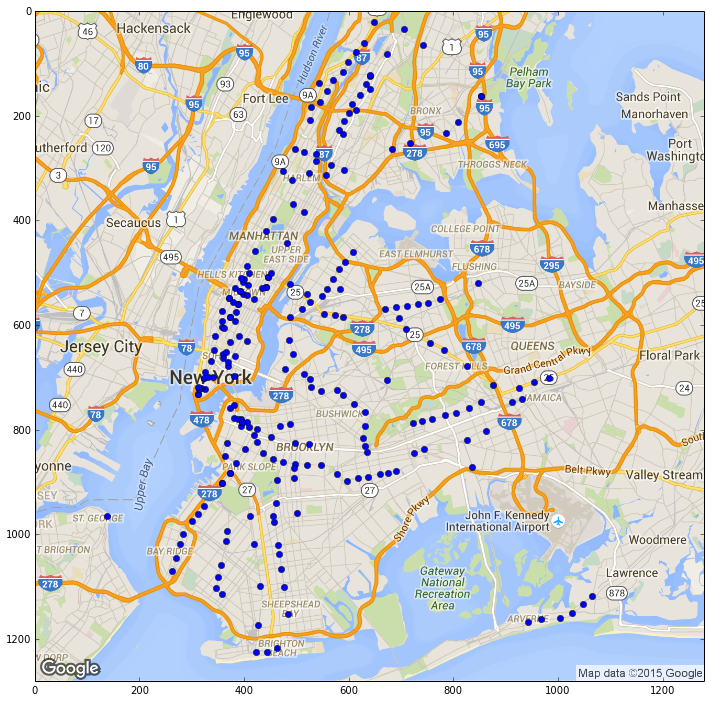
\includegraphics[width=\textwidth]{map_stations.png}
\caption{Map of NYC subway stations}
\label{fig:subway_stations}
\end{figure}

\section{Meteorology}

\subsection{Meteorologic stations and their regions of responsibility}

The weather at the the subway UNITs is measured by meteo stations, located in the UNITs' vicinity. There are 37 meteorologic stations. A given meteo station can service one or more UNITs, and each UNIT is serviced by exactly one meteo station.

Although not required for this project, an effort was made to visualize also the location of the meteo stations. This was done together with calculating a theoretical \textbf{region of responsibility} for each station. The idea of this region is to determine which subway UNITs should be serviced by which meteo station. This calculation was done by performing a Voronoi tessellation of the mesh formed by the meteo stations. Figure \ref{fig:meteo_voronoi} shows these regions in a color-coded way. Additionally, it shows again the subway UNITs, this time color-coding them with the color of their servicing meteo station (as reported by the dataset). We see that most UNITs (not all!) have the same color as the Voronoi region in which they are located---this means that the Voronoi tessellation was a really good way to determine the extents of the area that is best served by a given meteo station. 

\begin{figure}[ht]
\centering
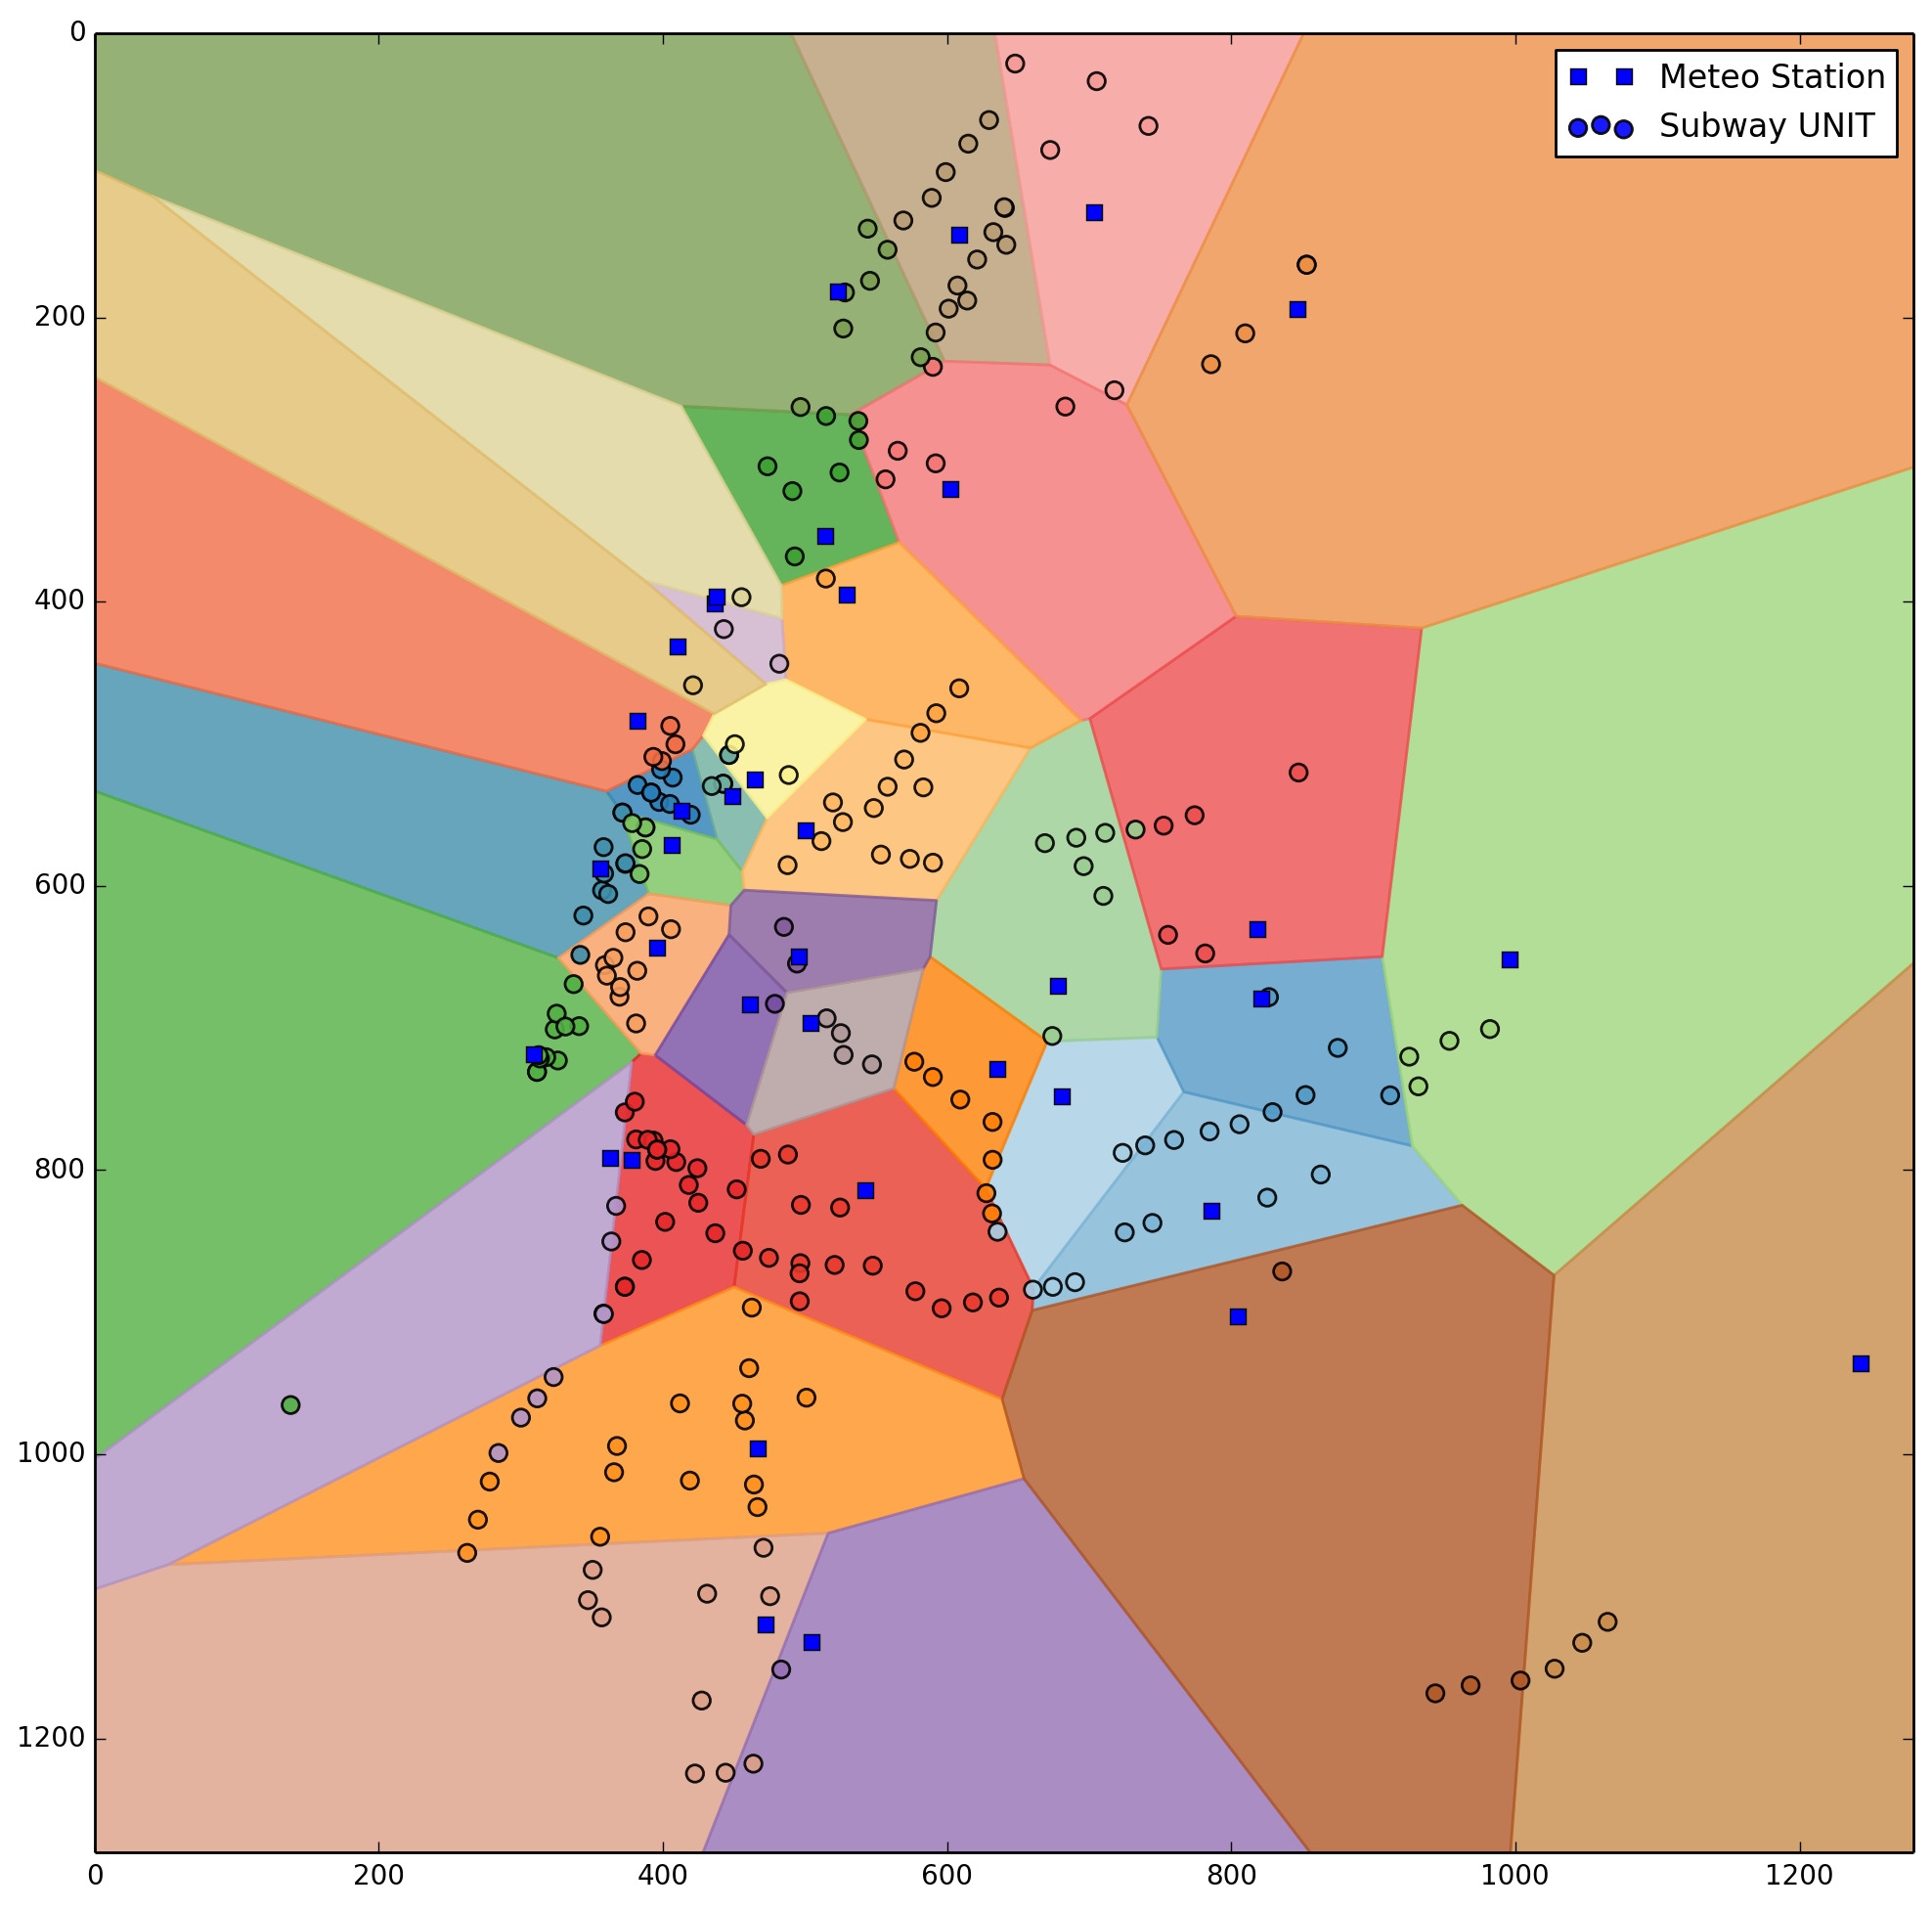
\includegraphics[width=\textwidth]{meteo_voronoi.png}
\caption{Map of NYC meteo stations, their Voronoi-calculated regions of responsibility and subway UNITs}
\label{fig:meteo_voronoi}
\end{figure}

\section{Meteorologic Conditions}

Using the Haversine geodesic formula (details in the IPython notebook), 
$$d = 2 r \arcsin \Bigg( \sqrt{ \sin^2 \bigg(\frac{\phi_2 - \phi_1} {2} \bigg) + \cos( \phi_2)\cos(\phi_1)\sin^2\bigg(\frac{\lambda_2 - \lambda_1} {2} \bigg) }\Bigg)$$
we find the \textbf{extents of the NYC subway area} to be approximately $35 \times 35 \ \rm km$. In this pretty big area we can expect to find different meteorologic conditions at different places at the same time.

Indeed, after performing some exploration with \tt pandas \rm of the initial dataset, we discover the following:
\begin{itemize}
\item It is possible for different subway stations to have different weather at the same point of time. For example, at the same moment there are stations having rain and others that do not.
\item There are 186 unique \tt datetime \rm points in the dataset (i.e. $31 \ \rm days \times 6 \ timepoints = 186$).
\item Of these 186 datetime points, there are 43 when some subway stations have been receiving rain, while others have not.
\item Of the remaining 143 datetime points, at 17 we've had all-rainy weather, and at 126---completely no-rain weather.
\item On '2011-05-19 04:00:00' we've had the most diversified rain conditions, i.e. almost half of the subway stations have been reporting rain, while the rest have been "dry". A map showing this can be seen in Figure \ref{fig:most-diverse-rain-conditions}
\item And now something \textbf{strange}---there are 459 records, that report both \emph{"Clear"} conditions and \emph{"Rain"}...
\end{itemize}







\end{document}
